\chapter{Gradle build configurations}
\label{chapter:gradle-build}

\begin{figure}[ht]
  \begin{center}
    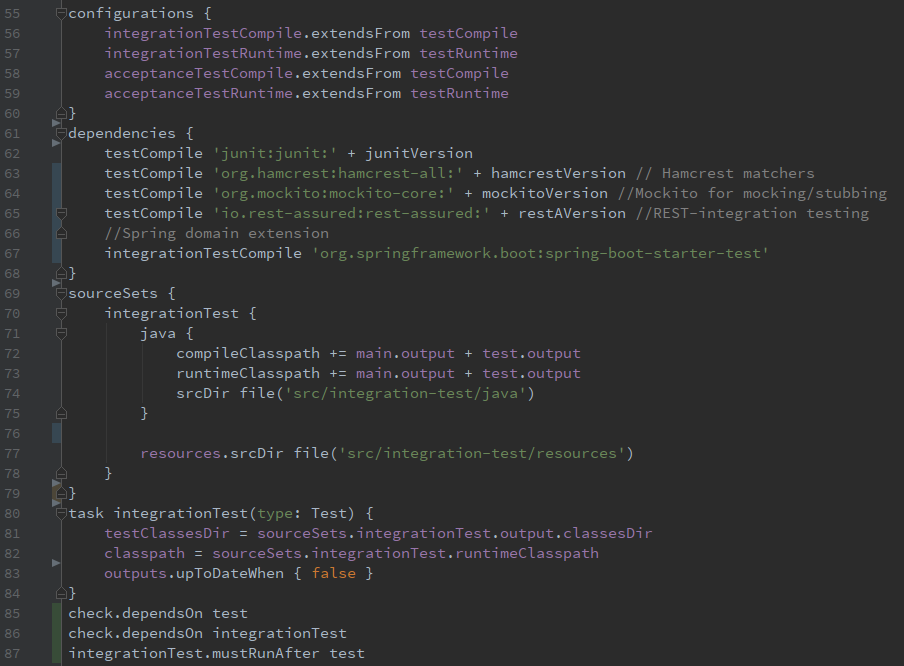
\includegraphics[width=13.7cm]{images/junit-build.png}
    \caption{Relevant parts of JUnit Gradle build configuration}
    \label{fig:junit-build}
  \end{center}
\end{figure}

\begin{figure}[ht]
  \begin{center}
    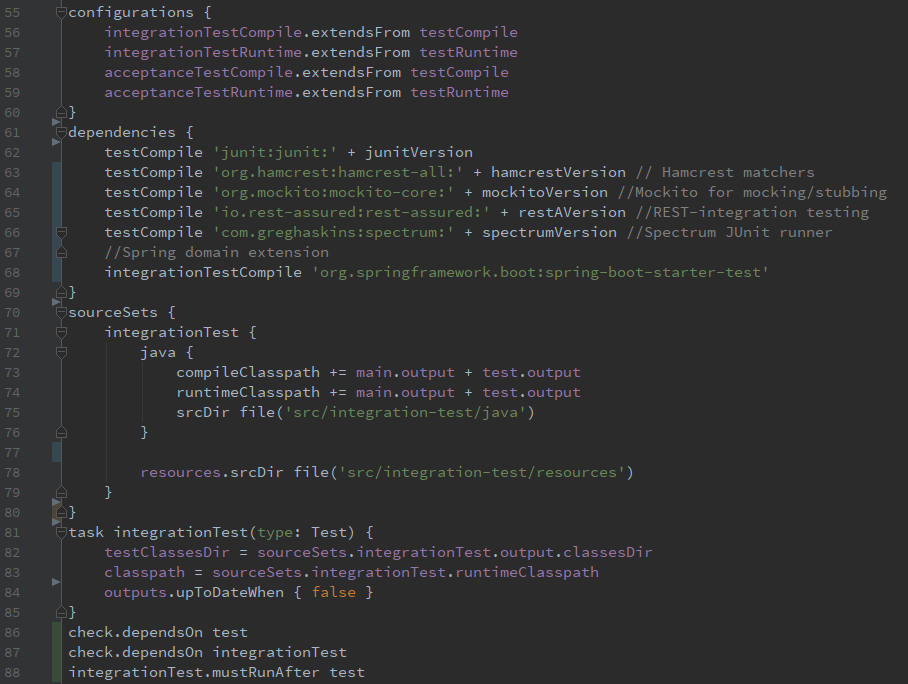
\includegraphics[width=13.7cm]{images/spectrum-build.png}
    \caption{Relevant parts of Spectrum Gradle build configuration}
    \label{fig:spectrum-build}
  \end{center}
\end{figure}

\begin{figure}[ht]
  \begin{center}
    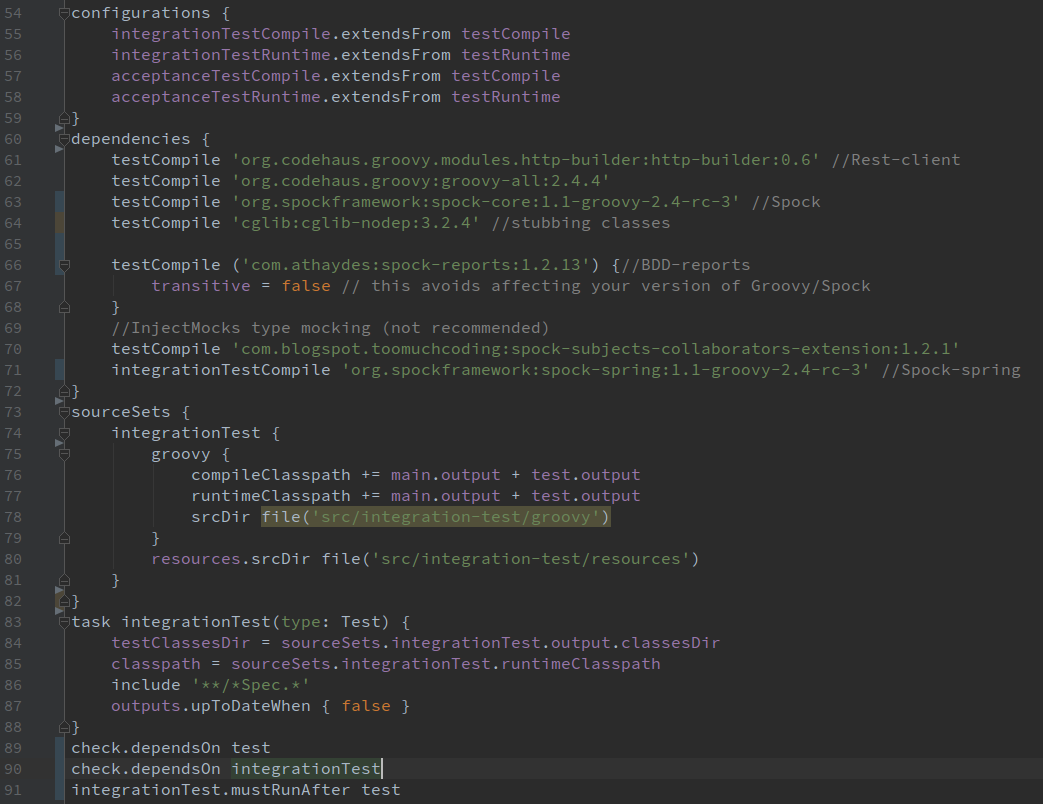
\includegraphics[width=13.7cm]{images/spock-gradle.png}
    \caption{Relevant parts of Spock Gradle build configuration}
    \label{fig:spock-build}
  \end{center}
\end{figure}

\begin{figure}[ht]
  \begin{center}
    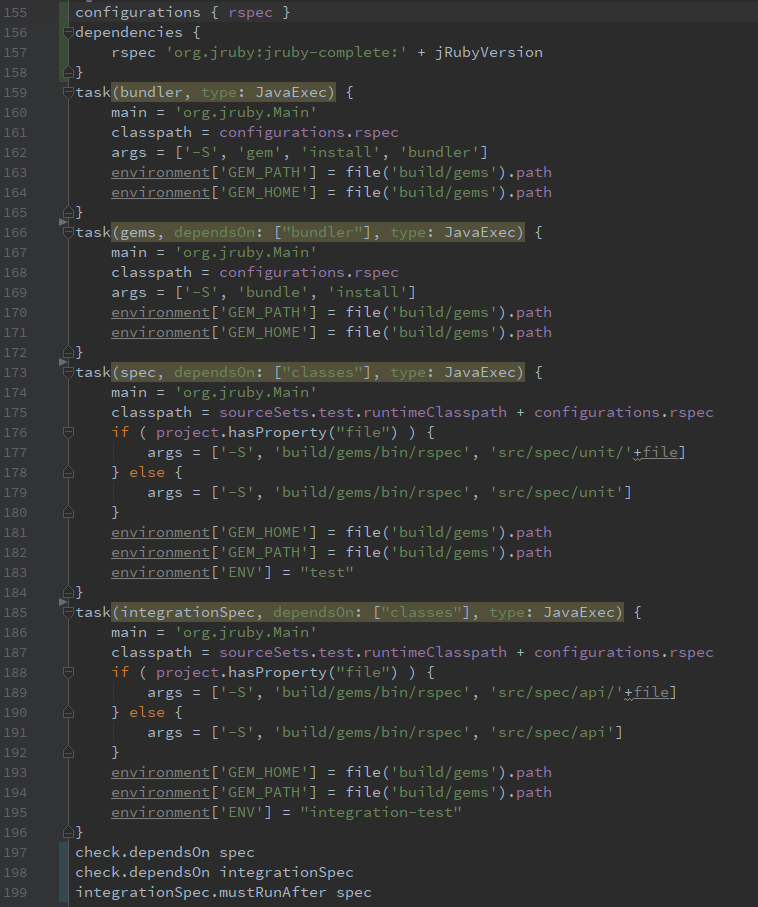
\includegraphics[width=13.7cm]{images/rspec-build.png}
    \caption{Relevant parts of RSpec Gradle build configuration}
    \label{fig:rspec-build}
  \end{center}
\end{figure}

\chapter{Interview questions}
\label{chapter:interview}
\section{Interview for demographic purposes}
    \label{section:demographic}
    \begin{outline}[enumerate]
    \1 How long have you worked as a software developer?
    \1 How long have you worked as a Java developer?
        \2 How long in the Spring Framework context?
    \1 What is the project you are working on now?
        \2 What is the context of project?
            \3 Industry branch or government related?
            \3 What is the nature of software development?
        \2 Does the project use agile or traditional process?
        \2 What is the size of the project?
        \2 What is the size of development team?
        \2 How would you describe the project's software architecture?
        \2 What practices are in the used quality assurance process?
        \2 What is the used automated testing framework for
            \3 Unit-level?
            \3 Integration-level?
    \1 How much experience do you have with automated
        \2 Unit testing and with what frameworks?
        \2 Integration testing and with what frameworks?
    \1 How much experience do you have with automated behavior driven development testing frameworks before this experiment?
    \1 What are your expectations regardings the switch to a new testing framework?
    \end{outline}

\newgeometry{top=1.5cm, bottom=1.5cm}
\chapter{Surveys}
\label{chapter:surveys}
This appendix explains in detail the two surveys used in this case study: their questions and relationship to related
research surveys \& found problems. First the survey regarding JUnit is examined, followed by the inspection of BDD testing
framework survey.
\section{Survey regarding JUnit in automated low level testing}
\label{section:junit-survey}
Survey regarding JUnit contains base questions from multiple previous research studies~\cite{williams2009effectiveness}~\cite{daka2014survey}~\cite{li2016automatically}.
They were used as base to see how the participants in this study are positioned related to other studied practitioners.
Related research in chapter \ref{chapter:background} section \ref{section:research} highlighted findings from previous studies.
This survey is aimed to study about the participants practices and perception related to common problems and other findings found in earlier research.
Table \ref{tab:junit-survey} displays how JUnit survey questions are related to previous studies and to which research questions
they will later help answering:
{\renewcommand{\arraystretch}{1.3}
\begin{table}[H]
    \resizebox{\textwidth}{!}{%
        \begin{tabular}{p{4.0cm}p{4.0cm}p{9.0cm}}
        \hline
        \textbf{Related research questions} & \textbf{Survey questions} & \textbf{Related research findings} \\ \hline
        RQ1 & Q3 & Developers are mainly trying to find realistic scenarios on what to test~\cite{daka2014survey} \\
        RQ1 & Q11, Q12 & Developers finding isolating of unit under test hard~\cite{daka2014survey} \\
        RQ2 & Q14 & Only half of the survey respondents enjoy writing unit tests~\cite{daka2014survey}~\cite{runeson2006survey} \\
        RQ1, RQ2 & Q2, Q7, Q14, Q15 & Maintaining unit tests was found hard~\cite{daka2014survey}~\cite{runeson2006survey} \\
        RQ1 & Q4, Q5, Q6 & For 60.38\% of developers, understanding unit tests is at least moderately difficult~\cite{li2016automatically} \\
        RQ1 & Q8, Q9 & Developers find updated documentation and comments in test cases useful, but writing comments to unit tests is rarely or never done~\cite{li2016automatically} \\
        RQ2 & Q14, Q15 & Majority of developers find unit tests helpful in producing higher quality code~\cite{williams2009effectiveness} \\
        RQ2 & Q14 & Majority of developers find unit tests helpful in understanding other peoples code~\cite{williams2009effectiveness} \\
        RQ1 & Q1, Q10 & \\
        RQ2 & Q16 & \\ \hline
        \end{tabular}}
        \caption {JUnit survey questions related to research questions and earlier studies} \label{tab:junit-survey}
\end{table}
}
\restoregeometry
Tables \ref{tab:junit-pt1}, \ref{tab:junit-pt2} and \ref{tab:junit-pt3} display all the questions in the JUnit survey.
They contain multiple copied questions from other
studies. All the copied questions originally had the word \textit{'unit'} in them instead of \textit{'low level'}. This change
was made to accompany both unit and integration testing into the survey of this study.

First copied questions are questions \textbf{Q1:} \textit{How do you spend your software development time?} and
\textbf{Q3:} \textit{How important are the following aspects for you when you write new low level tests?}~\cite{daka2014survey}.
These questions were copied to study as a base how the development time is used and what aspects are priortized in low level testing.
Q3 Subquestions 1 and 3-8 are originals. Q3 Subquestion 2 is added to this survey to study the initial attitude towards describing behavior
in tests.

Third copied question is \textbf{Q4:} \textit{How difficult is it for you usually to understand a low level test?}~\cite{li2016automatically}.
This question was added to survey to get a general concensus about understandability of the low level testing within participants.
Fourth and fifth copied questions are \textbf{Q8:} \textit{How often do you add/write documentation comments to low level test cases?} and
\textbf{Q9:} \textit{When you make changes to low level tests, how often do you comment the changes (or update existing comments)?}~\cite{li2016automatically}.
These questions were copied to study the low level testing documentation practices.

Sixth and seven copied questions are \textbf{Q14 \& Q15:} \textit{Please indicate your level of agreement with the following statements}.
Q14 and its subquestions 1-5 are copied from \textit{"A survey on unit testing practices and problems"} by Daka and Fraser~\cite{daka2014survey}.
Subquestions 6-8 are original questions defined in this thesis. Q15 subquestion 1 is copied from a unit test practitioner
survey done at Microsoft~\cite{williams2009effectiveness} and subquestion 2 is copied from unit test documentation
practices survey by Li et al.~\cite{li2016automatically}. Questions Q14 \& Q15 were copied to gather developer perception
towards low level testing.


\clearpage
\newgeometry{left=1cm, right=1cm}
    \begin{table}
        \resizebox{\textwidth}{!}{%
            \begin{tabular}{p{20.0cm}*{7}{p{2.0cm}}}
            \hline
            \textbf{Question} & \textbf{Answer options} &  &  &  &   &  & \\ \hline
            \textbf{Q1: How do you spend your software development time (in percentages)} & & & & & & \\
            & 0-100\% & & & & & & \\
            1. Writing new code &  \\
            2. Writing new tests &  \\
            3. Debugging/fixing &  \\
            4. Refactoring &  \\
            5. Other &  \\
            & \\ \hline

            \textbf{Q2: How do you spend your low level automated testing time} & & & & & & \\
             & minutes / 0-100\% & & & & & & \\
            1. How much approximately you use time per test case (minutes)? & \\
            2. How much of your initial effort goes to thinking about test case content without implementation (percentage)? & \\
            3. How much of your initial effort goes to initial test case structuring and implementation (percentage)? & \\
            4. How much of your overall testing effort goes to refactoring test code (percentage)? \\
            & \\ \hline

            \textbf{Q3: How important are the following aspects for you when you write new low level tests?} & & & & & & \\
            & Not at all & Low \newline importance & Slightly important & Neutral & Moderately important & Very \newline important & Extremely important \\
            1. Code coverage & \\
            2. Capturing all behavior of unit/feature with tests or assertions & \\
            3. Execution speed & \\
            4. Robustness against code changes (i.e., test does not break easily) & \\
            5. How realistic the test scenario is	& \\
            6. How easily faults can be localised/debugged if the test fails & \\
            7. How easily the test can be updated when the underlying code changes & \\
            8. Sensitivity against code changes (i.e., test should detect even small code changes) & \\
            & \\ \hline

            & & & & & & \\
            & Very easy & Easy & Moderate & Hard & Very hard & & \\
            \textbf{Q4: How difficult is it for you to understand a low level test?} & \\
            & \\ \hline

            \textbf{Q5: In low level testing, how difficult is it for you to} & & & & & & \\
            & Very easy & Easy & Slightly easy & Moderate & Slightly hard & Hard & Very hard \\
            1. Structure and write information to context of test? & \\
            2. Structure and write information to stimulus of test? & \\
            3. Structure and write information to assertions of test? & \\
            4. Read test case structure for information about context of test? & \\
            5. Read test case structure for information about stimulus of test? & \\
            6. Read test case structure for information about assertions of test? & \\
            & \\ \hline

            & & & & & & \\
            & Not at all & Hardly informative & Slightly informative & Somewhat informative & Moderately informative & Very informative & Extremely informative \\
            \textbf{Q6: How informative you usually find the test case output?} & \\
            & \\ \hline

            \textbf{Q7: How much are the following repetition reducing techniques used in your low level testing?} & & & & & & \\
            & Never & Very rarely & Rarely & Occasionally & Frequently & Very \newline frequently & Always \\
            1. Extract method (custom helper methods) & \\
            2. Lifecycle hooks Before/After -class & \\
            3. Lifecycle hooks Before/After (each) & \\
            4. Automatic test case generation via test case parametrization & \\
            5. Common test initializer class inheritance & \\
            & \\ \hline

            & & & & & & \\
            & Never & Rarely & Moderate & Hard & Very hard & & \\
            \textbf{Q8: How often do you add/write documentation comments to low level test cases?} & \\
            & \\ \hline

            & & & & & & \\
            & Never & Rarely & Moderate & Hard & Very hard & & \\
            \textbf{Q9: When you make changes to low level tests, how often do you comment the changes (or update existing comments)?} & \\
            & \\ \hline

            \textbf{Q10: In unit testing, how many} & & & & & & \\
            & 0 & 1 & 2-3 & 4-5 & 6-7 &  8-9 & 10 or more \\
            1. Test methods do you usually write per class method? & \\
            2. Assertions do you usually write per test method? & \\
            & \\ \hline

            & & & & & & \\
            & Mockito & jMock & Powermock & Easymock & Other & & \\
            \textbf{Q11: In unit testing, what mocking library do you normally use?} & \\
            & \\ \hline

            \textbf{Q12: In unit testing, how difficult you find it to} & & & & & & \\
            & Very easy & Easy & Slightly easy & Moderate & Slightly hard & Hard & Very hard \\
            1. Mock objects? & \\
            2. Stub method calls? & \\
            3. Verify mock object actions? \\
            & \\ \hline

            & & & & & & \\
            & Before implementation & During implementation & After implementation & \\
            \textbf{Q13: When do you add automated unit tests for developed code?} & \\
            & \\ \hline

            \end{tabular}}
            \caption {JUnit developer low level testing practice questions} \label{tab:junit-pt1}
    \end{table}
    \clearpage
    \begin{table}[H]
        \resizebox{\textwidth}{!}{%
            \begin{tabular}{p{20.0cm}*{7}{p{2.0cm}}}
            \hline
            \textbf{Question} & \textbf{Answer options} &  &  &  &   &  & \\ \hline

            \textbf{Q14: Please indicate your level of agreement with the following statements} & & & & & & \\
            & Strongly disagree & Disagree & Somewhat disagree & Neither agree nor disagree & Somewhat agree & Agree & Strongly agree \\
            1. Writing low level tests is difficult &  \\
            2. I enjoy writing low level tests &  \\
            3. I would like to have more tool support when writing low level tests &  \\
            4. I would like to have more low level tests &  \\
            5. Maintaining low level tests is difficult &  \\
            6. I think my low level tests will help other developers to understand the implemented unit/feature better & \\
            7. Low level automated testing helps me find defects in the code before other quality assurance phases & \\
            8. JUnit promotes me to write high quality test code & \\
            & \\ \hline

            \textbf{Q15: Please indicate your level of agreement with the following statements} & & & & & & \\
            & Strongly disagree & Disagree & Neutral & Agree & Strongly agree & \\
            1. Overall, low level tests help me produce higher quality code &  \\
            2. Maintaining good low level test cases and their documentations is important to the quality of a system &  \\
            & \\ \hline

            \end{tabular}}
            \caption {Likert scale questions of developer perception towards JUnit} \label{tab:junit-pt2}
    \end{table}
    \vspace{20px}
    \begin{table}[H]
        \resizebox{\textwidth}{!}{%
            \begin{tabular}{p{17.0cm}*{11}{p{1.55cm}}}
            \hline
            \textbf{Question} & \textbf{Answer options} &  &  &  &  &  &  &  &  & \\ \hline

            \textbf{Q16: How likely are you to} &  &  &  &  &  &  &  &  &  &  \\
            & 0 & 1 & 2 & 3 & 4 & 5 & 6 & 7 & 8 & 9 & 10 \\
            1. Recommend low level automated testing for colleague as a software development practice? &  \\
            2. Recommend testing framework JUnit for future Spring projects where you take part in existing project? &  \\
            3. Take testing framework JUnit in use for future Spring projects where you have technical lead role in a new starting project? & \\
            & \\ \hline

            \end{tabular}}
            \caption {NPS questions of developer loyalty towards low level automated testing with JUnit} \label{tab:junit-pt3}

    \end{table}
    \clearpage
\restoregeometry






\section{Survey regarding BDD testing framework in automated low level testing}
\label{section:bdd-survey}
Survey regarding BDD testing framework was aimed for the projects A and B explained in chapter \ref{chapter:projects}. This means
that for project A, the survey was aimed at to study the differences between JUnit and \textit{xSpec family} testing done with \textbf{Spectrum}.
For project B, survey was targeted to study the change from JUnit to \textit{Gherkin family} \textbf{Spock} testing framework.
BDD testing framework survey questions together with base JUnit survey questions are used to answer to researh questions
RQ1 and RQ2. Table \ref{tab:bdd-survey} demonstrates how BDD testing framework survey questions are related to previous research findings
and research questions in this thesis:

{\renewcommand{\arraystretch}{1.3}
\begin{table}[H]
    \resizebox{\textwidth}{!}{%
        \begin{tabular}{p{4.0cm}p{4.0cm}p{9.0cm}}
        \hline
        \textbf{Related research questions} & \textbf{Survey questions} & \textbf{Related research findings} \\ \hline
        RQ1 & Q3' & Developers are mainly trying to find realistic scenarios on what to test~\cite{daka2014survey} \\
        RQ1 & Q11', Q12' & Developers finding isolating of unit under test hard~\cite{daka2014survey} \\
        RQ2 & *Q14' & Only half of the survey respondents enjoy writing unit tests~\cite{daka2014survey}~\cite{runeson2006survey} \\
        RQ1, RQ2 & Q2', Q7', *Q14', Q15 & Maintaining unit tests was found hard~\cite{daka2014survey}~\cite{runeson2006survey} \\
        RQ1 & Q4', Q5', Q6', Q15 & For 60.38\% of developers, understanding unit tests is at least moderately difficult~\cite{li2016automatically} \\
        RQ1 & Q8', Q9' & Developers find updated documentation and comments in test cases useful, but writing comments to unit tests is rarely or never done~\cite{li2016automatically} \\
        RQ2 & *Q14' & Majority of developers find unit tests helpful in producing higher quality code~\cite{williams2009effectiveness} \\
        RQ2 & *Q14', Q15 & Majority of developers find unit tests helpful in understanding other peoples code~\cite{williams2009effectiveness} \\
        RQ1 & Q1', Q10' & \\
        RQ2 & Q16' & \\ \hline
        \end{tabular}}
        \caption {JUnit survey questions related to research questions and earlier studies}
        \caption* {* = Q14' contains direct comparison to JUnit survey questions Q14 and Q15}
        \label{tab:bdd-survey}
\end{table}
}

Questions marked with '-character are direct comparison questions to question with same number in JUnit survey displayed
in section \ref{section:junit-survey}. For example original question \textbf{Q2} in JUnit survey:
\textit{"How do you spend your low level automated testing time?"} has its direct comparison question \textbf{Q2'}:
\textit{"Compared to JUnit, How do you spend your low level automated testing time?"}. Although there were individual surveys
used for each Spock and Spectrum, their questions are both displayed in same tables. The only change is in the words
\textit{Spectrum/Spock}, which are marked in questions. Full questions used in BDD surveys are displayed in tables \ref{tab:spock-spectrum-pt1},
\ref{tab:spock-spectrum-pt2}, \ref{tab:spock-spectrum-pt3} and \ref{tab:spock-spectrum-pt4}.

\newgeometry{left=1cm, right=1cm}
    \begin{table}
        \resizebox{\textwidth}{!}{%
            \begin{tabular}{p{18.0cm}*{7}{p{2.4cm}}}
            \hline
            \textbf{Question} & \textbf{Answer \newline options} &  &  &  &   &  & \\ \hline

            \textbf{Q1': Compared to JUnit, How do you spend your software development time?} & & & & & & \\
            & A lot less time & Less time & Slightly less time & The same amount & Slightly more time & More time & A lot more time \\
            1. Writing new code &  \\
            2. Writing new tests &  \\
            3. Debugging/fixing &  \\
            4. Refactoring &  \\
            5. Other &  \\
            & \\ \hline

            \textbf{Q2': Compared to JUnit, How do you spend your low level automated testing time?} & & & & & & \\
            & A lot less & Less & Slightly less & The same amount & Slightly more & More & A lot more \\
            1. Do you use more or less time per test case? & \\
            2. Do you use more or less of initial effort thinking about test case content? (no implementation) & \\
            3. Do you use more or less of initial effort to test case structuring and implementation? & \\
            4. Do you use more or less of overall testing effort to refactoring test code? \\
            & \\ \hline

            \textbf{Q3': Compared to JUnit, How important are the following aspects for you when you write new low level tests?} & & & & & & \\
            & A lot less important & Less important & Slightly less important & As important as before & Slightly more important & More important & A lot more important \\
            1. Code coverage & \\
            2. Capturing all behavior of unit/feature with tests or assertions & \\
            3. Execution speed & \\
            4. Robustness against code changes (i.e., test does not break easily) & \\
            5. How realistic the test scenario is	& \\
            6. How easily faults can be localised/debugged if the test fails & \\
            7. How easily the test can be updated when the underlying code changes & \\
            8. Sensitivity against code changes (i.e., test should detect even small code changes) & \\
            & \\ \hline

            & & & & & & \\
            & A lot less difficult & Less difficult & Slightly less difficult & As difficult as before & Slightly more difficult & More difficult & A lot more difficult \\
            \textbf{Q4': Compared to JUnit, how difficult is it for you to understand a low level test?} & \\
            & \\ \hline

            \textbf{Q5': Compared to JUnit in low level testing, how difficult is it for you to.} & & & & & & \\
            & A lot less difficult & Less difficult & Slightly less difficult & As difficult as before & Slightly more difficult & More difficult & A lot more difficult \\
            1. Structure and write information to context of test? & \\
            2. Structure and write information to stimulus of test? & \\
            3. Structure and write information to assertions of test? & \\
            4. Read test case structure for information about context of test? & \\
            5. Read test case structure for information about stimulus of test? & \\
            6. Read test case structure for information about assertions of test? & \\
            & \\ \hline

            & & & & & & \\
            & A lot less informative & Less informative & Slightly less informative & As informative as before & Slightly more informative & More informative & A lot more informative \\
            \textbf{Q6': Compared to JUnit, how informative you usually find the test case output?} & \\
            & \\ \hline

            \textbf{Q7': Compared to JUnit, how much are the following repetition reducing techniques used in your low level testing?} & & & & & & \\
            & A lot less & Less & Slightly less & The same amount & Slightly more & More & A lot more \\
            1. Extract method (custom helper methods) & \\
            2. Lifecycle hooks Before/After -class & \\
            3. Lifecycle hooks Before/After (each) & \\
            4. Automatic test case generation via test case parametrization & \\
            5. Common test initializer class inheritance & \\
            & \\ \hline

            & & & & & & \\
            & A lot less & Less & Slightly less & The same amount & Slightly more & More & A lot more \\
            \textbf{Q8': Compared to JUnit, how often do you add/write documentation comments to low level test cases?} & \\
            & \\ \hline

            & & & & & & \\
            & A lot less & Less & Slightly less & The same amount & Slightly more & More & A lot more \\
            \textbf{Q9': Compared to JUnit when you make changes to low level tests, how often do you comment the changes (or update existing comments)?} & \\
            & \\ \hline

            \textbf{Q10': Compared to JUnit in unit testing} & & & & & & \\
            & A lot less & Less & Slightly less & The same amount & Slightly more & More & A lot more \\
            1. Do you write more or less test methods per class method? & \\
            2. Do you write more or less assertions per test method? & \\
            & \\ \hline

            & & & & & & \\
            & Mockito & jMock & Powermock & Easymock & Other & \textit{Spock's internal mocking} & \\
            \textbf{Q11': In unit testing with \textit{Spectrum/Spock}, what mocking library do you normally use?} & \\
            & \\ \hline

            \textbf{Q12': Compered to JUnit in unit testing, how difficult you find it to} & & & & & & \\
            & A lot easier & Easier & Slightly easier & As difficult as before & Slightly harder & Harder & A lot harder \\
            1. Mock objects? & \\
            2. Stub method calls? & \\
            3. Verify mock object actions? \\
            & \\ \hline

            & & & & & & \\
            & Before implementation & During implementation & After implementation & \\
            \textbf{Q13': When do you add automated unit tests for developed code?} & \\
            & \\ \hline

            \end{tabular}}
            \caption {\textit{Spectrum/Spock} developer low level testing practice questions} \label{tab:spock-spectrum-pt1}
    \end{table}
    \clearpage
    \begin{table}[H]
        \resizebox{\textwidth}{!}{%
            \begin{tabular}{p{20.0cm}*{7}{p{2.0cm}}}
            \hline
            \textbf{Question} & \textbf{Answer options} &  &  &  &   &  & \\ \hline

            \textbf{Q14': Please indicate your level of agreement with the following statements} & & & & & & \\
            & Strongly disagree & Disagree & Somewhat disagree & Neither agree nor disagree & Somewhat agree & Agree & Strongly agree \\
            1. Writing low level tests with \textit{Spectrum/Spock} is more difficult than with JUnit &  \\
            2. I enjoy writing low level tests with \textit{Spectrum/Spock} more than I do with JUnit &  \\
            3. I would like to have more tool support for \textit{Spectrum/Spock} when writing low level tests &  \\
            4. I would like to have more low level tests for \textit{Spectrum/Spock} &  \\
            5. Maintaining low level tests with \textit{Spectrum/Spock} is more difficult than with JUnit &  \\
            6. I think my low level tests with \textit{Spectrum/Spock} will help other developers to understand the implemented unit/feature better than earlier tests with JUnit & \\
            7. Low level automated testing with \textit{Spectrum/Spock} helps me find defects in the code before other quality assurance phases better than earlier tests with JUnit & \\
            8. \textit{Spectrum/Spock} promotes me to write higher quality test code than with JUnit & \\
            9. Overall, low level tests with \textit{Spectrum/Spock} help me produce higher quality code than with JUnit & \\
            10. Maintaining good low level test cases and their documentation with \textit{Spectrum/Spock} is more important for system quality than maintaining JUnit test cases & \\
            & \\ \hline

            \end{tabular}}
            \caption {Likert scale questions of developer perception towards \textit{Spectrum/Spock}} \label{tab:spock-spectrum-pt2}
    \end{table}

    \vspace{20px}
    \begin{table}[H]
        \resizebox{\textwidth}{!}{%
            \begin{tabular}{p{15.0cm}*{3}{p{2.0cm}}}
            \hline
            \textbf{Question} & \textbf{Answer options} &  &  \\ \hline

            \textbf{Q15: I would say that I write more} &  &  & \\
            & Yes & Uncertain & No \\
            1. Understandable low level tests with \textit{Spectrum/Spock} than with JUnit? &  \\
            2. Maintainable low level tests with \textit{Spectrum/Spock} than with JUnit? &  \\
            & \\ \hline

            \end{tabular}}
            \caption {Questions of developer perception towards \textit{Spectrum/Spock}} \label{tab:spock-spectrum-pt3}

    \end{table}


    \vspace{20px}
    \begin{table}[H]
        \resizebox{\textwidth}{!}{%
            \begin{tabular}{p{17.0cm}*{11}{p{1.55cm}}}
            \hline
            \textbf{Question} & \textbf{Answer options} &  &  &  &  &  &  &  &  & \\ \hline

            \textbf{Q16': How likely are you to} &  &  &  &  &  &  &  &  &  &  \\
            & 0 & 1 & 2 & 3 & 4 & 5 & 6 & 7 & 8 & 9 & 10 \\
            1. Recommend low level automated testing for colleague as a software development practice? &  \\
            2. Recommend testing framework \textit{Spectrum/Spock} for future Spring projects where you take part in existing project? &  \\
            3. Take testing framework \textit{Spectrum/Spock} in use for future Spring projects where you have technical lead role in a new starting project? & \\
            & \\ \hline

            \end{tabular}}
            \caption {NPS questions of developer loyalty towards low level automated testing with \textit{Spectrum/Spock}} \label{tab:spock-spectrum-pt4}
    \end{table}

\clearpage
    \begin{table}
        \resizebox{\textwidth}{!}{%
            \begin{tabular}{p{20.0cm}*{7}{p{2.0cm}}}
            \hline
            \textbf{Question} & \textbf{Answer options} &  &  &  &   &  & \\ \hline
            \textbf{Q1: How do you spend your software development time (in percentages)} & Participant A & Participant B & Participant C & Average & & \\
            & & & & & & & \\
            1. Writing new code & 20\% & 40\% & 15\% & 25\%  \\
            2. Writing new tests & 20\% & 25\% & 20\% & 21.67\% \\
            3. Debugging/fixing & 30\% & 25\% & 25\% & 26.67\% \\
            4. Refactoring & 20\%  & 10\% & 30\% & 23.33\% \\
            5. Other & 10\% & 0\% & 10\% & 6.67\% \\
            & \\ \hline


            \textbf{Q2: How do you spend your low level automated testing time} & Participant A & Participant B & Participant C & Average & & \
            & & & & & & & \\
            1. How much approximately you use time per test case (minutes)? & 30 min & 30 min & 30 min & 30 min \\
            2. How much of your initial effort goes to thinking about test case content without implementation (percentage)? & 50\% & 20\% & 15\% & 28.33\% \\
            3. How much of your initial effort goes to initial test case structuring and implementation (percentage)? & 50\% & 80\% & 85\% & 71.67\% \\
            4. How much of your overall testing effort goes to refactoring test code (percentage)? & 50\% & 5\% & 30\% & 28.33\% \\
            & \\ \hline

            \textbf{Q3: How important are the following aspects for you when you write new low level tests?} & & & & & & \\
            & Not at all & Low \newline importance & Slightly important & Neutral & Moderately important & Very \newline important & Extremely important \\
            1. Code coverage & 0 & 0 & 0 & ABC & 0 & 0 & 0 \\
            2. Capturing all behavior of unit/feature with tests or assertions & 0 & 0 & B & A & 0 & C & 0 \\
            3. Execution speed & 0 & C & 0 & 0 & B & A & 0 \\
            4. Robustness against code changes (i.e., test does not break easily) & 0 & 0 & 0 & 0 & ABC & 0 & 0 \\
            5. How realistic the test scenario is & 0 & 0 & AB & 0 & 0 & C & 0 \\
            6. How easily faults can be localised/debugged if the test fails & 0 & 0 & B & 0 & AC & 0 & 0 \\
            7. How easily the test can be updated when the underlying code changes & 0 & C & A & 0 & B & 0 & 0 \\
            8. Sensitivity against code changes (i.e., test should detect even small code changes) & 0 & AB & 0 & C & 0 & 0 & 0 \\
            & \\ \hline

            & & & & & & \\
            & Very easy & Easy & Moderate & Hard & Very hard & & \\
            \textbf{Q4: How difficult is it for you to understand a low level test?} & 0 & 0 & BC & A & 0 \\
            & \\ \hline

            \textbf{Q5: In low level testing, how difficult is it for you to} & & & & & & \\
            & Very easy & Easy & Slightly easy & Moderate & Slightly hard & Hard & Very hard \\
            1. Structure and write information to context of test? & 0 & A & 0 & 0 & BC & 0 & 0 \\
            2. Structure and write information to stimulus of test? & 0 & 0 & 0 & ABC & 0 & 0 & 0 \\
            3. Structure and write information to assertions of test? & 0 & B & C & 0 & A & 0 & 0 \\
            4. Read test case structure for information about context of test? & 0 & 0 & C & 0 & B & A & 0 \\
            5. Read test case structure for information about stimulus of test? & 0 & 0 & C & B & A & 0 & 0 \\
            6. Read test case structure for information about assertions of test? & 0 & B & C & 0 & 0 & A & 0 \\
            & \\ \hline

            & & & & & & \\
            & Not at all & Hardly informative & Slightly informative & Somewhat informative & Moderately informative & Very informative & Extremely informative \\
            \textbf{Q6: How informative you usually find the test case output?} & 0 & A & 0 & C & B & A & 0 \\
            & \\ \hline

            \textbf{Q7: How much are the following repetition reducing techniques used in your low level testing?} & & & & & & \\
            & Never & Very rarely & Rarely & Occasionally & Frequently & Very \newline frequently & Always \\
            1. Extract method (custom helper methods) & 0 & 0 & 0 & 0 & AB & C & 0 \\
            2. Lifecycle hooks Before/After -class & 0 & 0 & 0 & C & AB & 0 & 0 \\
            3. Lifecycle hooks Before/After (each) & 0 & 0 & 0 & 0 & AB & C & 0 \\
            4. Automatic test case generation via test case parametrization & 0 & A & B & C & 0 & 0 & 0 \\
            5. Common test initializer class inheritance & 0 & AC & B & 0 & 0 & 0 & 0 \\
            & \\ \hline

            & & & & & & \\
            & Never & Rarely & Sometimes & Fairly often & Always & & \\
            \textbf{Q8: How often do you add/write documentation comments to low level test cases?} & 0 & C & 0 & AB & 0 \\
            & \\ \hline

            & & & & & & \\
            & Never & Rarely & Sometimes & Fairly often & Always & & \\
            \textbf{Q9: When you make changes to low level tests, how often do you comment the changes (or update existing comments)?} & 0 & C & 0 & AB & 0 \\
            & \\ \hline

            \textbf{Q10: In unit testing, how many} & & & & & & \\
            & 0 & 1 & 2-3 & 4-5 & 6-7 &  8-9 & 10 or more \\
            1. Test methods do you usually write per class method? & 0 & 0 & AB & C & 0 & 0 & 0 \\
            2. Assertions do you usually write per test method? & 0 & 0 & AB & C & 0 & 0 & 0 \\
            & \\ \hline

            & & & & & & \\
            & Mockito & jMock & Powermock & Easymock & Other & & \\
            \textbf{Q11: In unit testing, what mocking library do you normally use?} & ABC & 0 & 0 & 0 & 0 \\
            & \\ \hline

            \textbf{Q12: In unit testing, how difficult you find it to} & & & & & & \\
            & Very easy & Easy & Slightly easy & Moderate & Slightly hard & Hard & Very hard \\
            1. Mock objects? & 0 & BC & A & 0 & 0 & 0 & 0 \\
            2. Stub method calls? & 0 & 0 & AC & 0 & B & 0 & 0 \\
            3. Verify mock object actions? & 0 & BC & 0 & A & 0 & 0 & 0 \\
            & \\ \hline

            & & & & & & \\
            & Before implementation & During implementation & After implementation & \\
            \textbf{Q13: When do you add automated unit tests for developed code?} & 0 & BC & A \\
            & \\ \hline

            \end{tabular}}
            \caption {JUnit developer low level testing practice questions with response data} \label{tab:junit-pt1-ans}
    \end{table}
    \clearpage
    \begin{table}[H]
        \resizebox{\textwidth}{!}{%
            \begin{tabular}{p{20.0cm}*{7}{p{2.0cm}}}
            \hline
            \textbf{Question} & \textbf{Answer options} &  &  &  &   &  & \\ \hline

            \textbf{Q14: Please indicate your level of agreement with the following statements} & & & & & & \\
            & Strongly disagree & Disagree & Somewhat disagree & Neither agree nor disagree & Somewhat agree & Agree & Strongly agree \\
            1. Writing low level tests is difficult & 0 & 0 & C & 0 & AB & 0 & 0 \\
            2. I enjoy writing low level tests & 0 & B & 0 & A & 0 & C & 0 \\
            3. I would like to have more tool support when writing low level tests & 0 & 0 & B & A & C & 0 & 0 \\
            4. I would like to have more low level tests & 0 & 0 & 0 & ABC & 0 & 0 & 0 \\
            5. Maintaining low level tests is difficult & 0 & 0 & C & 0 & B & A & 0 \\
            6. I think my low level tests will help other developers to understand the implemented unit/feature better & 0 & 0 & B & 0 & A & C & 0 \\
            7. Low level automated testing helps me find defects in the code before other quality assurance phases & 0 & 0 & 0 & 0 & B & C & A \\
            8. JUnit promotes me to write high quality test code & 0 & 0 & AC & B & 0 & 0 & 0 \\
            & \\ \hline

            \textbf{Q15: Please indicate your level of agreement with the following statements} & & & & & & \\
            & Strongly disagree & Disagree & Neutral & Agree & Strongly agree & \\
            1. Overall, low level tests help me produce higher quality code & 0 & 0 & 0 & B & AC \\
            2. Maintaining good low level test cases and their documentations is important to the quality of a system & 0 & 0 & 0 & AB & C \\
            & \\ \hline

            \end{tabular}}
            \caption {Likert scale questions with response data about developer perception towards JUnit} \label{tab:junit-pt2-ans}
    \end{table}
    \vspace{20px}
    \begin{table}[H]
        \resizebox{\textwidth}{!}{%
            \begin{tabular}{p{17.0cm}*{11}{p{1.55cm}}}
            \hline
            \textbf{Question} & \textbf{Answer options} &  &  &  &  &  &  &  &  & \\ \hline

            \textbf{Q16: How likely are you to} &  &  &  &  &  &  &  &  &  &  \\
            & 0 & 1 & 2 & 3 & 4 & 5 & 6 & 7 & 8 & 9 & 10 \\ \hline
            1. Recommend low level automated testing for colleague as a software development practice? & 0 & 0 & 0 & 0 & 0 & 0 & 0 & 0 & B & 0 & AC \\
            2. Recommend testing framework JUnit for future Spring projects where you take part in existing project? & 0 & 0 & 0 & 0 & 0 & 0 & 0 & C & 0 & B & A \\
            3. Take testing framework JUnit in use for future Spring projects where you have technical lead role in a new starting project? & 0 & 0 & 0 & 0 & 0 & 0 & 0 & 0 & C & B & A \\
            & \\ \hline

            \end{tabular}}
            \caption {NPS questions with response data about developer loyalty towards low level automated testing with JUnit } \label{tab:junit-pt3-ans}

    \end{table}
    \clearpage

\restoregeometry



